\chapter{Architectural Design} \label{ch:architectural_design}


\section{Overview}
 At the high level, the system employs a client-server architecture. The client part consists of the web application running in a browser on a user's machine, whereas the server part is composed of web, DREAM, mail, and SQL servers. The high-level architecture is presented in the figure \ref{fig:high-level-architecture}.

\begin{figure}[H]
    \centering
    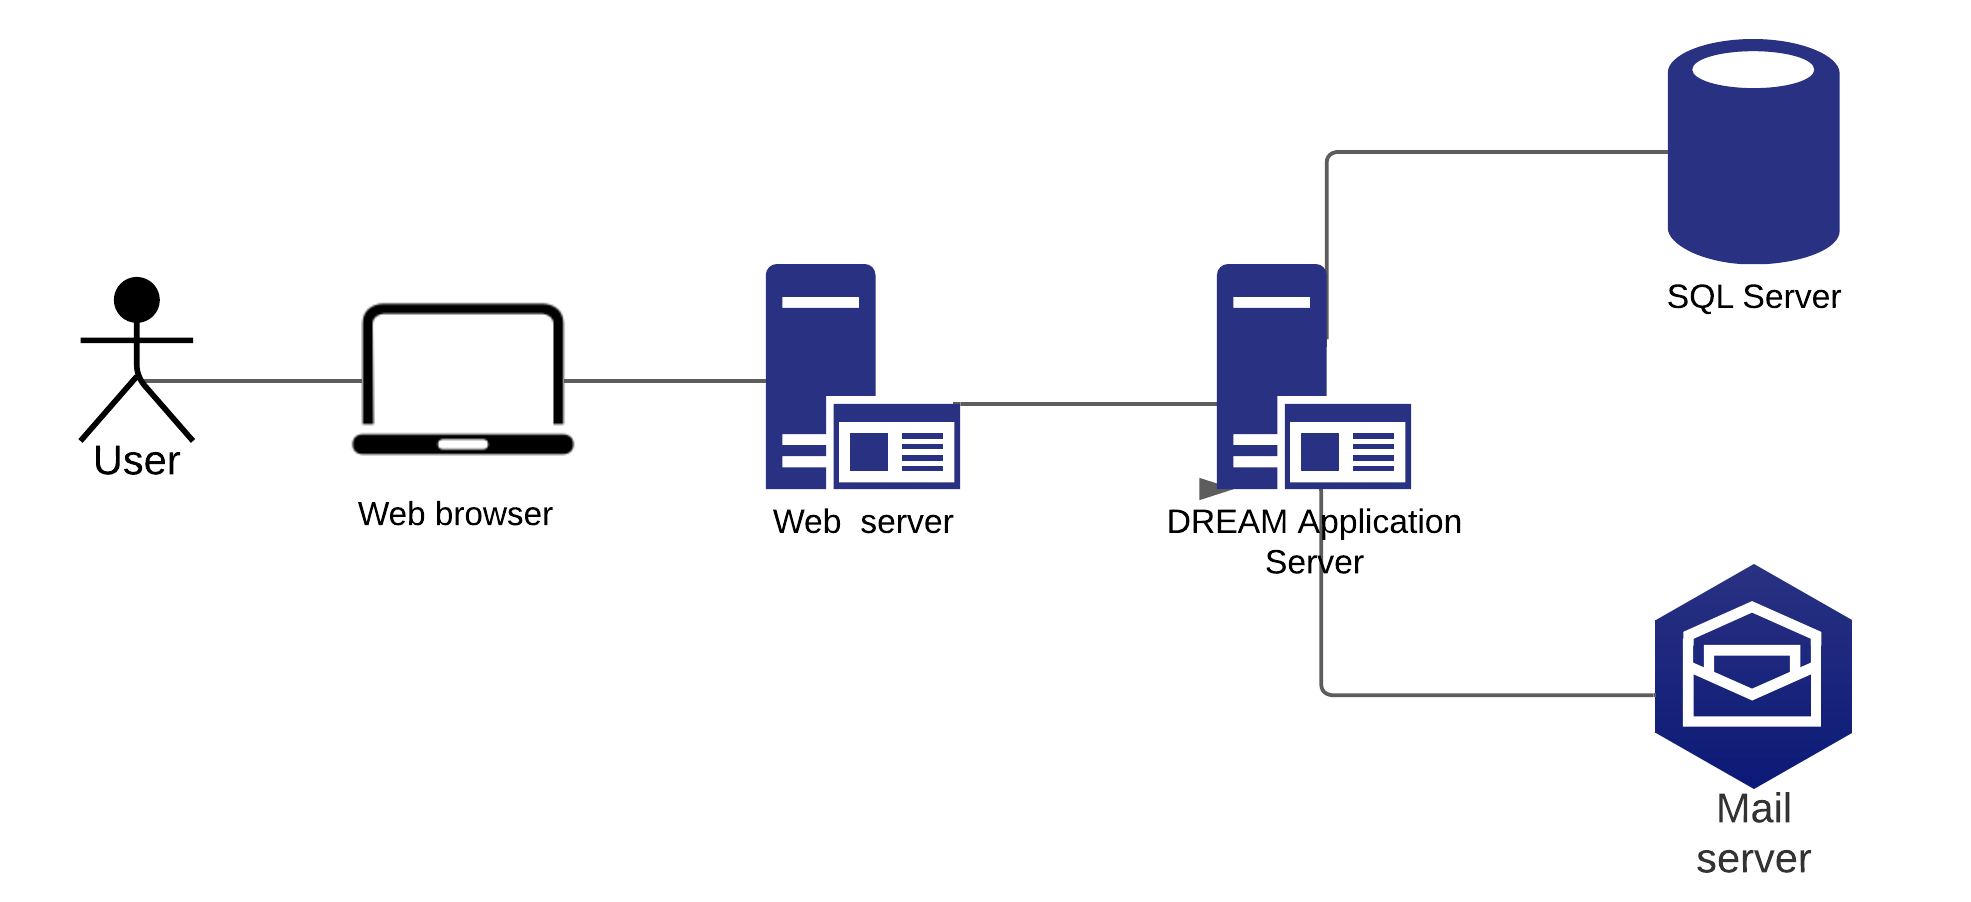
\includegraphics[width=12cm, height=6cm]
    {figures/Overview.png}
    \caption{High-level architecture diagram}
    \label{fig:high-level-architecture}
\end{figure}

The DREAM server part uses a database hosted on a SQL Server to store data collected from the users as well as external systems, and the Mail Server used to send the emails required for password reset. Moreover, the web server works as a middleware between the user interface and the database, utilizing HTTP protocol to receive and respond to requests from the web application running on a client's web browser. Finally, the \textit{DREAM server} hosts the application server (\textit{backend} part) with the majority of the application business logic. 

\section{Component View}

\subsection{High level}
\todo{add high level diagram}

\subsection{DREAM server}\label{subsec:backend-components}
Detailed component diagram of the DREAM Server is presented in the figure \ref{fig:backend-components}. The server application was broken down into 3 layers using N-tiers architecture pattern described in section \ref{sec:patterns}. The communication between layers is established by implementation of interfaces presented in the diagram. In accordance with the N-tier pattern, the communication runs only in one direction – starting from the API layer down to the Data Access layer. 

\begin{figure}[H]
    \centering
    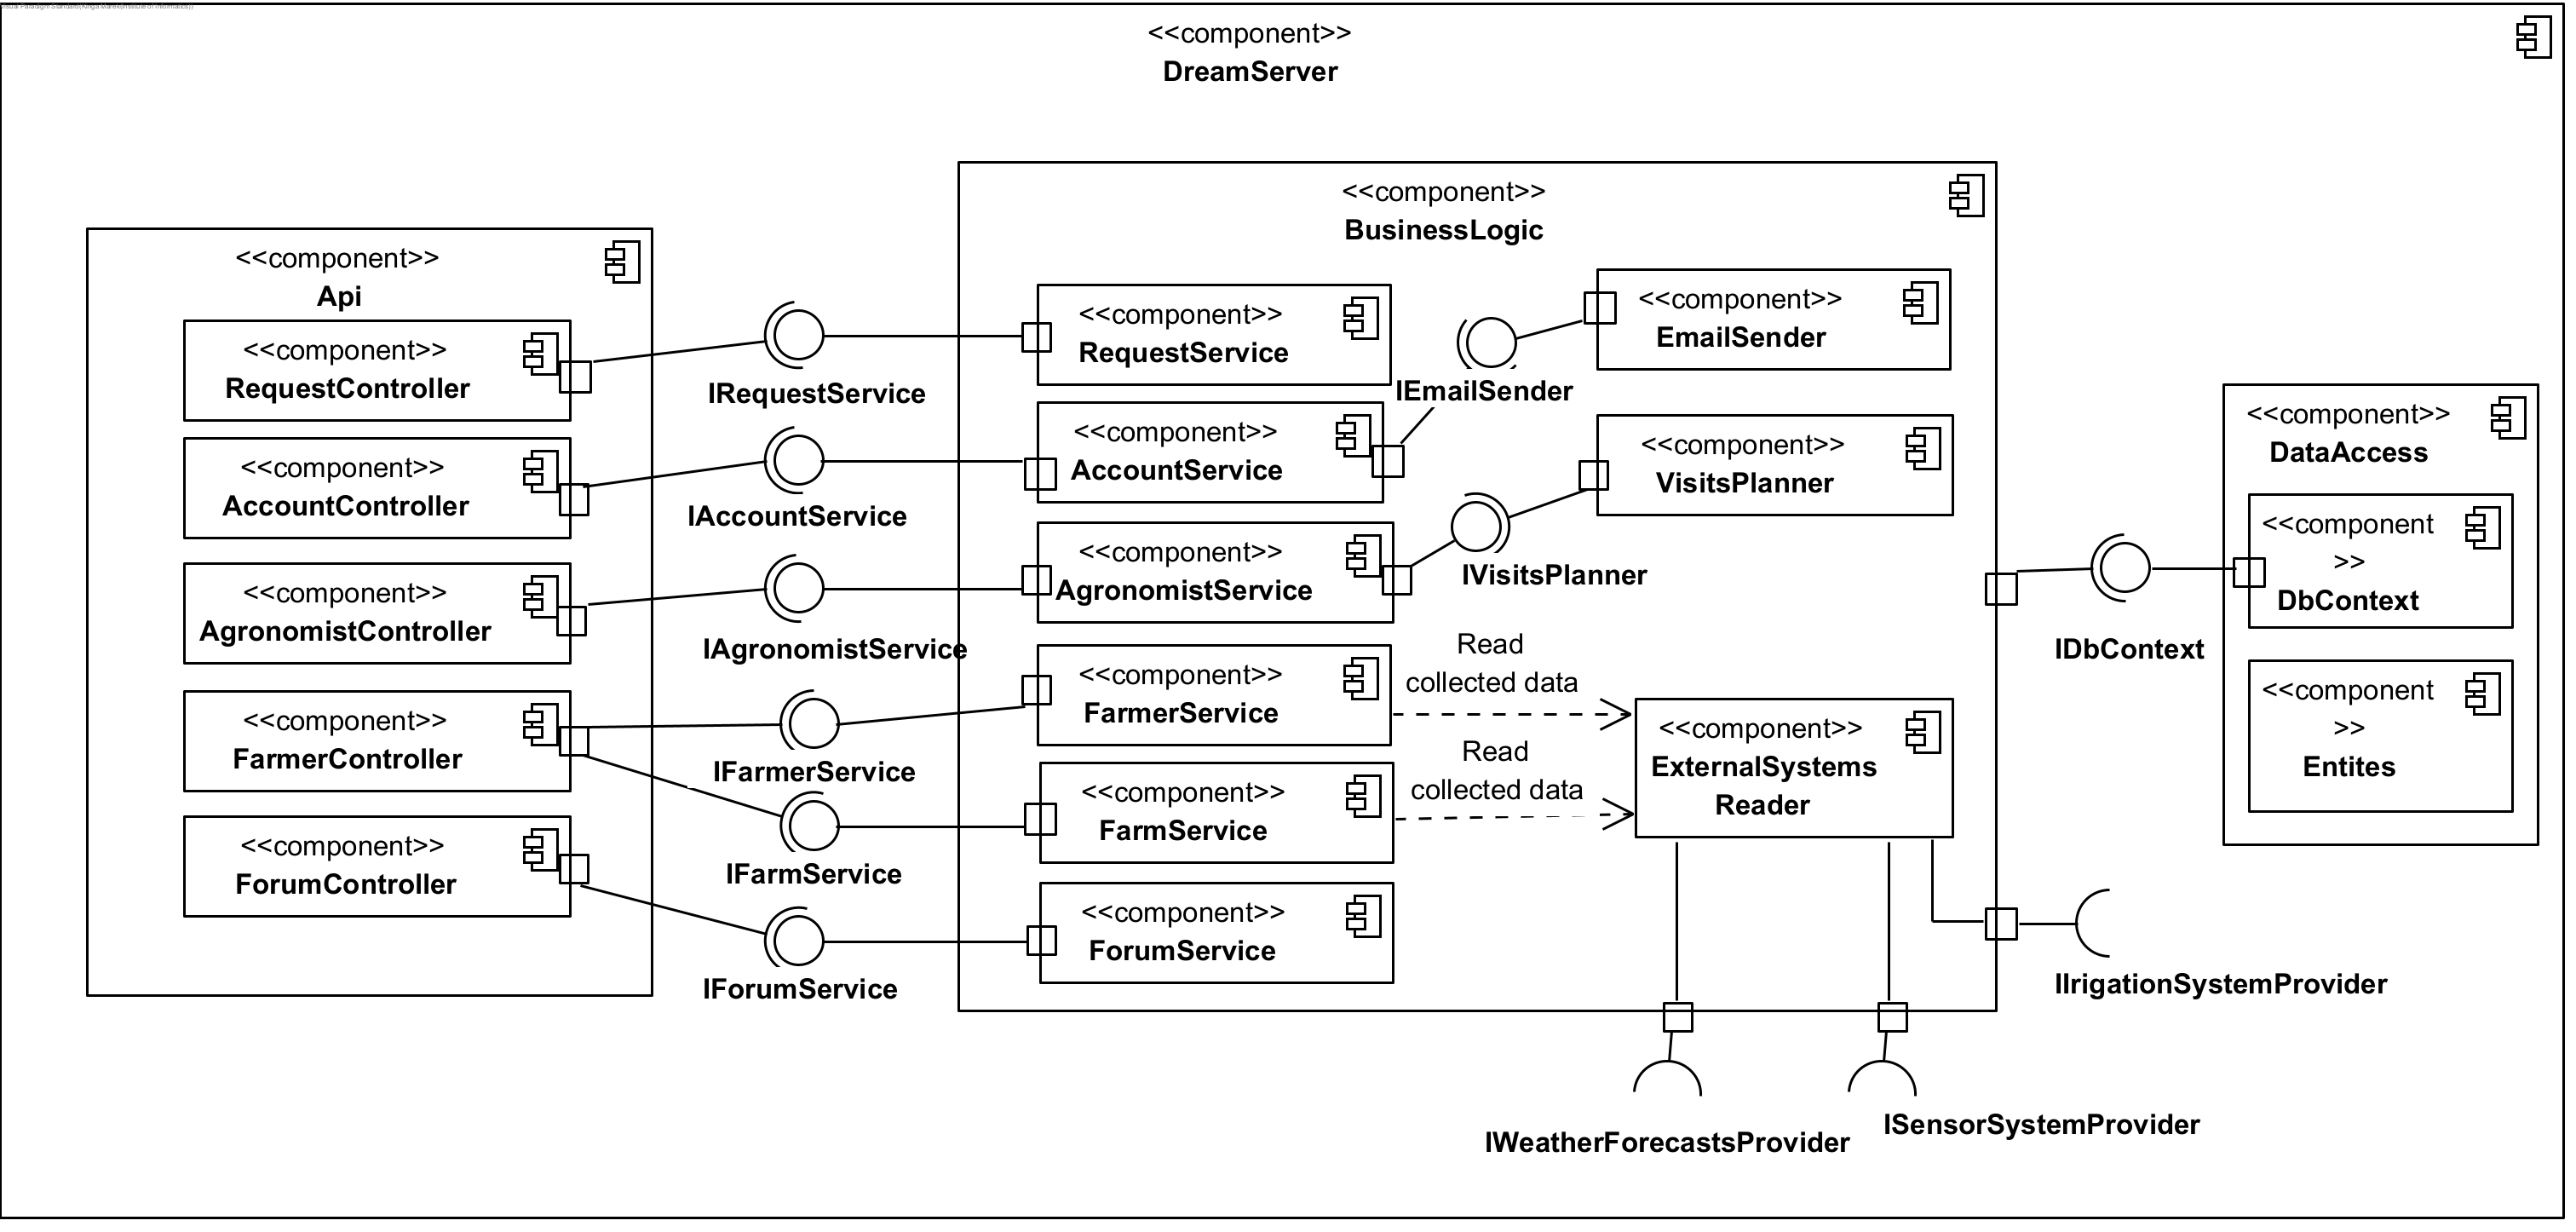
\includegraphics[scale=0.58, origin=c]
    {diagrams/component/BackendComponents.png}
    \caption{DREAM server component diagram}
    \label{fig:backend-components}
\end{figure}

The first layer, the API layer, is composed by a set of controllers that describe available REST endpoints. Then, the middle layer, Business Logic layer contains services and other classes that provide logic necessary for handling requests \todo{Do you mean help requests or requests? It is unclear given the following context} from the client application and cooperation with external systems. In detail, the Business logic layer contains:
\begin{itemize}
    \item \textbf{RequestService} - handles creating, editing, deleting and accessing help requests together with logic required for automatic selection of requests' recipients.
    \item \textbf{AccountService} - handles account registration and deletion, password reset and authentication logic.
    \item \textbf{AgronomistService} - handles area of responsibility and daily plan management, setting execution state of visits. It calls VisistsPlanner about the necessities to plan new visits after each submission of daily plan execution state or rejection of planned visit.
    \item \textbf{FarmerService} - handles notes assignment and providing data required for building farmer's summary (access to notes history). Moreover, retrieves personalized suggestions for the farmer based on his farm's location and production type.
    \item \textbf{FarmService} - handles management of farmers' production data, providing data required for building farmer's summary (farm's external systems and  production data).  
    \item \textbf{ForumService} - handles accessing and creating forum threads; accessing, creating and deleting comments.
    \item \textbf{EmailSender} - handles logic required for e-mail sending during password reset process.
    \item \textbf{VisitsPlanner} - handles implementation of \textit{visits scheduling algorithm} described in subsection \ref{subsec:visits-alg}.
    \item \textbf{ExternalSystemsReader} - handles logic required for execution of daily jobs that read and store in the database data obtained from IWeatherForecastsProvider, ISensorSystemProvider and IIrigationSystemProvider interfaces. The implementation of these interfaces is provided by the external systems' API. 
\end{itemize}

Finally, the Data Access layer contains entities and classes required to efficiently communicate with the database. The components of this layer were not presented in detail, as the communication with the database will leverage object relational mapping described in \todo{Implementation chapter, entity framework}.

\section{Deployment View}
\begin{figure}[H]
    \centering
    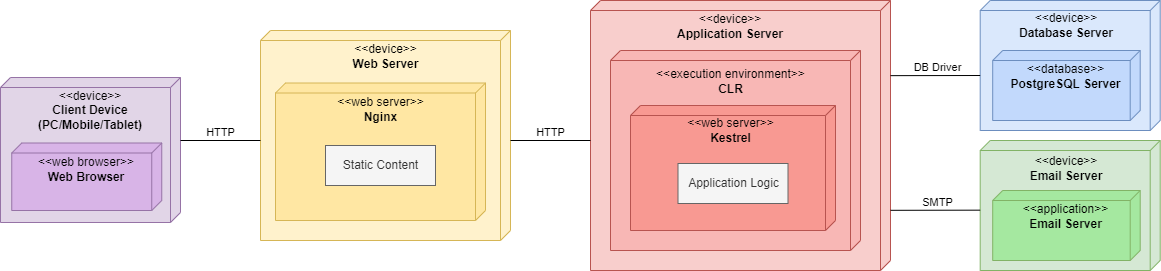
\includegraphics[width=\textwidth]{diagrams/deployment.png}
    \caption{Deployment diagram}
    \label{fig:deployment}
\end{figure}
The system is divided into 5 parts: 3 main tiers \todo{inne słowo} (Application Server, Web Server, Database Server), Client Device with Web Browser and Email Server.
\begin{itemize}
    \item \textbf{Application Server} - DREAM backend server, it handles application logic and provides a REST API \cite{rest}. It runs using Kestrel Web Server, which is loaded by Common Language Runtime (CLR), the virtual machine component of Microsoft .NET Framework \todo{Missing references}
    \item \textbf{Web Server} - DREAM frontend server, it provides the user interface layer. It hosts the static version of the website using Nginx \cite{nginx}. The website communicates with the Application Server tier via REST API using HTTP requests.
    \item \textbf{Database Server} - Database storage system, using PostgreSQL \cite{postgresql}. It allows data access using DB driver. 
    \item \textbf{Client Device} - Device used by clients to access the website hosted in Web Server tier using HTTP requests. It can be any type of device, capable of running a modern web browser
    \item \textbf{Email Server} - Email server, allowing to send messages via SMTP protocol.
\end{itemize}


\section{Runtime View}

\section{Component Interfaces}

\section{Selected Architectural Styles and Patterns}\label{sec:patterns}
\begin{itemize}
    \item \textbf{Client Server} - a pattern, which enforces the principle of separation of concerns, by separating the service requesters (clients) from the providers of a resource or service (servers). Clients and servers communicate over a network and can be hosted on separate hardware.
    \item \textbf{REST} (\textit{Representational State Transfer}) – the API hosted on a DREAM server should be prepared using the REST API design rules \cite{rest} \cite{rest-microsoft}. Firstly, it should not bind the client application to any specific implementation by utilizing HTTP as the communication protocol. Furthermore, as it was presented in the DREAM server components diagram in subsection \ref{subsec:backend-components}, additional layers will be introduced to the server side application to avoid direct dependencies of the API on the database model. Additionally, the interface should be resource-oriented and the HTTP verbs \todo{czym są HTTP verbs?} should reflect the operations done on the resources. All this aims at improving the maintainability, reusability, and readability of the server application.
    \item \textbf{N-tier application} – the server side application was divided into 3 layers: API, Business Logic, and Data Access. This architecture was adopted following the types of common web application architectures described in Microsoft's documentation \cite{ntier}. However, the \textit{User Interface} layer was replaced by \textit{API} layer to better present its meaning. The choice was motivated by the simplicity of the architecture compared to other architectures like \textit{Clean architecture} or microservices architecture. 
    \item \textbf{Dependency Injection} - a dependency inversion technique that focuses on providing the implementation of required interfaces instead of creating them explicitly by the dependent objects. The main reason for introduction of this principle is the need to address the difficulty of testing the business logic layer \cites{ntier} \cite{di}. \todo{move it to the implementation chapter?}
\end{itemize}

\section{Other Design Decisions}

\subsection{Visit Scheduling Algorithm}\label{subsec:visits-alg}

One of the most important features of the system is the ability to schedule agronomist's visits to a farm. Requirement \textbf{R5} (all the requirements are described in RASD) states that all farms must be visited at least twice a year, whereas \textbf{R14} extends it further by adding a constraint that under-performing farmer's, meaning farmers with a negative note, should be visited more often, depending on the problem they are facing.

The system must be therefore able to schedule visits to a farm in a way that satisfies both requirements. This section presents an overview of the algorithm employed to tackle this problem.

\subsubsection*{General approach}

When planning a new visit it is necessary to take the following factors into consideration:
\begin{itemize}
    \item dates and number of already planned visits to the farm,
    \item number of visits planned for an agronomist on a given day,
    \item type of the problem the farmer is facing.
\end{itemize}

Function \textit{calculateVisitsToAdd} presented in the listing \ref{lst:CalculateVisitsToAdd} calculates the number of visits to add to the farm, given the number of already planned visits to the farm, the number of visits planned for an agronomist on a given day and the type of the problem the farmer is facing. In case there are already more visits to the farm planned than the number of casual visits (2) and the number of visits to add, then no new visit is necessary and the function returns 0. Such situation may happen when there are many visits planned to one farm due to the agronomist's decision.

\lstinputlisting[language=Cpp, caption={Function calculating the number of visits to add due to a problem.}, label={lst:CalculateVisitsToAdd}]{algorithms/visit_scheduling/CalculateVisitsToAdd.cpp}

Another function, presented in the listing \ref{lst:GetOptimalVisitDate} is \textit{getOptimalVisitDate}. It finds the greatest gap between two consecutive visits to the farm and inserts a new visit in between. It also considers a time slot in exactly one year from the current date, so that in case of completing a casual visit, a new one is created in approximately half of a year.

\lstinputlisting[language=Cpp, caption={Function responsible for picking the optimal date of a new visit.}, label={lst:GetOptimalVisitDate}]{algorithms/visit_scheduling/GetOptimalVisitDate.cpp}

\subsubsection*{Planning additional visits}

This section presents the process of scheduling a new visit to a farm. Function \textit{createVisitOnTheMostQuietDayCloseToDate} is presented in the listing \ref{lst:CreateVisitOnTheMostQuietDayCloseToDate}. It is responsible for creating a new visit to the farm on the most quiet day close to the date specified in the function's argument. It goes through up to 5 days before the proposed date and searches for an agronomist, who has not reached the maximum number of visits to the farm on a given day, otherwise, the visit is scheduled for the agronomist with the least visits planned in the specified window.

\lstinputlisting[language=Cpp, caption={Function creating a new visit on the most quiet day that is close to the specified date.}, label={lst:CreateVisitOnTheMostQuietDayCloseToDate}]{algorithms/visit_scheduling/CreateVisitOnTheMostQuietDayCloseToDate.cpp}

Function \textit{createAdditionalVisits}, presented in the listing \ref{lst:CreateAdditionalVisit}, is the main function responsible for scheduling additional visits to the farm.

\lstinputlisting[language=Cpp, caption={Function creating additional visits.}, label={lst:CreateAdditionalVisit}]{algorithms/visit_scheduling/CreateAdditionalVisit.cpp}

Due to the abovementioned requirements, the system must be able to schedule different types of visits to the farm. These types are identified by the visit's reason. The following listing \ref{lst:PlanVisits} presents the function meant to handle this problem.

\lstinputlisting[language=Cpp, caption={Function responsible for planning new visits.}, label={lst:PlanVisits}]{algorithms/visit_scheduling/PlanVisits.cpp}

\subsubsection*{Farmer registration}

Listing \ref{lst:CreateFarmer} presents the process of creating a farmer. Each time a new farmer is created, the system must plan two casual visits to his farm.

\lstinputlisting[language=Cpp, caption={Function responsible for creating a new farmer.}, label={lst:CreateFarmer}]{algorithms/visit_scheduling/CreateFarmer.cpp}

\subsubsection*{Daily plan submission}

Function \textit{updateVisit} (listing \ref{lst:UpdateVisit}) is responsible for changing the date of a visit. It is only possible to do so only if the new date is greater or equal than the current one. In case an agronomist wants to reschedule a visit that is casual, the system allows him to do so, but the date can be postponed only by a maximum of 5 days. Otherwise, the systems rejects the request and throws a warning.

\lstinputlisting[language=Cpp, caption={Function responsible for updating a visit.}, label={lst:UpdateVisit}]{algorithms/visit_scheduling/UpdateVisit.cpp}

The process of submitting a visit is described in the listing \ref{lst:SubmitVisit}. In case the date of a visit is greater than the current date, the visit is submitted. In case the date is less than the current date, a warning is thrown. A casual visit is a cyclic one, therefore a new one is scheduled every time its status becomes confirmed or rejected. In case of rejecting a casual visit, a new one is scheduled in the maximum of next 5 days following the process shown in the listing \ref{lst:PlanVisits}.

\lstinputlisting[language=Cpp, caption={Function responsible for submitting a visit.}, label={lst:SubmitVisit}]{algorithms/visit_scheduling/SubmitVisit.cpp}

\subsubsection*{Obtaining a negative note}

Every time a farmer's note changes from negative to neutral or positive, the system deletes all the visits to the farm that were planned due to the negative note. The function \textit{DeleteVisitsCreatedDueToNegativeNote} (listing \ref{lst:DeleteVisitsCreatedDueToNegativeNote}) handles that.

\lstinputlisting[language=Cpp, caption={Function that deletes visits created due to a negative note.}, label={lst:DeleteVisitsCreatedDueToNegativeNote}]{algorithms/visit_scheduling/DeleteVisitsCreatedDueToNegativeNote.cpp}

Function presented in the listing \ref{lst:SetNote} assures that every time a farmer receives a negative note, there are additional visits to his farm planned. The number of these visits depends on the type of the problem the farmer faces, which is priorly specified by a policy maker when assigning the note.

\lstinputlisting[language=Cpp, caption={Function responsible for setting the farmer's note.}, label={lst:SetNote}]{algorithms/visit_scheduling/SetNote.cpp}

\subsection{Database model}

\todo{Add a short description}

\begin{figure}[H]
    \centering
    \includegraphics
    [width=\textwidth]
    %[scale=0.45, origin=c]
    {figures/db-diagram.png}
    \caption{Database model}
    \label{fig:db-model}
\end{figure}

\begin{figure}[H]
    \centering
    \includegraphics
    [height = 0.9\textheight]
    %[scale=0.45, origin=c]
    {diagrams/database-model.png}
    \caption{Database model}
    \label{fig:db-model}
\end{figure}
